\chapter{Phylogenetic space}
To understand the challenges of assessing convergence of phylogenetic MCMC, it is desirable to describe the parameter space which it attempts to explore.
In this section I introduce the necessary technical background for a rigorous characterisation of phylogenetic space.
I will restrict attention to binary (bifurcating), rooted, labelled phylogenies.
First, it is convenient to define some notation.
The presentation will follow~\cite{Semple2003} for the general theory and~\cite{Drummond2002} for time-trees, with minor adjustments.

A rooted binary tree $t \in \boldsymbol T$ on $n$ taxa is a graph $G(V_t, E_t)$ with $2n-2$ edges, $n-2$ internal nodes and $n$ leaf/external nodes.
Each vertex (node) $v \in V_t$ has degree $3$, except for a special \textit{root} internal node, denoted $\rho$, which has degree $2$.
Each of the edges in $t$ can associated with a unique node numbering.
We can supplement $t$ with a set of branch lengths $\boldsymbol b = \{b_1, b_2, \ldots, b_{2n-2} \}$, $\boldsymbol b \in \boldsymbol B \subseteq \mathbb{R}_{+}^{2n-2}$.
Denote the object $(t, \boldsymbol b) = \tau \in \boldsymbol\Psi$.
For convenience, we will henceforth call $t$ a \textbf{topology} and $\tau$ a \textbf{phylogeny}.
Throughout this chapter I will use $\boldsymbol\Psi$ to denote the parameter space encompassing topologies and branch lengths,\textit{i.e.} the space of phylogenies, henceforth called ``phylogenetic space''.

In many applications, we are interested in placing the branching events represented by $t$ in absolute calendar time.
This leads to the construction of the central object of this chapter: time-calibrated phylogenies (TCP).
Specifically, since my main interest is in phylodynamic modelling, I will focus on phylogenies with~\textit{serially-sampled} tips (or taxa/leaves), where sequences are sampled through time and every terminal node -- corresponding to a sequence/taxon -- has a known sampling date.
For a node $i \in V$ let $a_i$ be the age of that node in calendar years.
A convenient labelling is to make labels increase with age, such that $i > j$ implies $a_i \geq a_j$.
Thus, the root node will have label $2n-1$.
Let $\boldsymbol L$ be the set of external/leaf nodes and let $\boldsymbol I$ be the set of internal nodes.
An edge $e_{i,j}$ with $i > j$ represents an ancestral lineage and node $k$ in $\boldsymbol I$ corresponds to a \textit{coalescence} event of two ancestral lineages at time $a_k$.
It is convenient to define $\boldsymbol a_L$ and $\boldsymbol a_L$ as the ages of the leaf and internal nodes, respectively.
Also denote $\boldsymbol a  = (\boldsymbol a_L , \boldsymbol a_I) \in \boldsymbol A \subset \mathbb{R}_+^{2n-1}$.
Note that here $\boldsymbol a_L$ is fixed (for any $t \in  \boldsymbol T$) as it relates to the data collection process. 

Lastly, we are then in position to define the set of \textbf{intercoalescent intervals} as $\boldsymbol s = \{s_2, s_3, \ldots, s_n\} \in \boldsymbol S \subset {R}_+^{n-1}$, where $s_i = a_{n-i+1}-a_{n-i}$ for $i = 2, \ldots, n-1$ and $s_n = a_1$.
Notice that for trees with tips sampled through time, $\boldsymbol s$ will have to be slightly adjusted to include subintervals that correspond to the intervals between either a coalescence or sampling event.
Finally, let $k_i$ denote the number of existing lineages in the interval $[a_{i-1}, a_i]$, $\boldsymbol k = \{k_2, k_3, \ldots, k_n\} \in \boldsymbol K \subset \mathbb{N}^{n-1}$.
Defining these quantities is important in that many prior distributions commonly used in Bayesian phylogenetics are based on coalescent processes and the measure of a phylogeny $\tau$ depends on it only through its coalescent intervals and numbers of lineages, $\boldsymbol s(\tau)$.
Notice there is a bijective mapping $H: \boldsymbol B \rightarrow \boldsymbol A$ that maps the branch lengths of a TCP to its node ages\footnote{Also sometimes called node heights.}.
An striking feature of the space of phylogenetic trees is its sheer size.
A well-known counting argument shows that there are $ |\boldsymbol T| = T(n) = 1 \times 3 \times \ldots \times (2n-5) \times (2n-3) = (2n-3)!!$ binary rooted phylogenies on $n \geq 3$ taxa.

For another useful representation of trees, one can also consider bipartitions of the leaves, called ``splits'' or ``clades''.%\footnote{Strictly speaking, splits are defined for unrooted phylogenies, while clades are used when discussing rooted phylogenies.}.
An example of a split is $\{A, B, C\} | \{ D, E\}$, where $A, B, C, D$ and $E$ are tips.
We will refer to the set of all possible splits on $n$ taxa as $\boldsymbol C$.
For $n \geq 3$ taxa, there are $|\boldsymbol C| = 2^{n-1}-1$ possible splits, and a given tree can contain at most $2n-2$ splits.
Two splits $U_1 | V_1$ and $U_2 | V_2$ are said to be \textit{compatible} iff at least one of the intersections $U_1 \cap U_2$, $U_1 \cap V_2$, $V_1 \cap U_2$ and $U_1 \cap U_2$ is empty.
Let $\boldsymbol C^\star \subset \boldsymbol C$ be  the space of pairwise compatible clades,~\textit{i.e.}, S $\boldsymbol x \in \boldsymbol C^\star$ iff all clades in $\boldsymbol x$ are pairwise compatible.

% One can use the concept of node height (see main text) to associate a height with each of the $n-1$ internal nodes in a rooted binary tree.
% These can then be ranked and then used to form a poset $\boldsymbol h^{\text{int}} = \{h_1^{\text{int}}, h_2^{\text{int}}, \ldots, h_{n-1}^{\text{int}}\} \in \boldsymbol H \subset \mathbb{R}_+^{n-1}$, with $h_i^{\text{int}} > h_{i-1}^{\text{int}}$.

% \begin{remark}
% \label{thm:TBtoS}
%  The mapping $g: (\boldsymbol T, \boldsymbol A) \to \boldsymbol S$ is non-injective surjective.
% \end{remark}
% 
% From the method of construction of the intercoalescent intervals, it is clear that there exists a bijection between $\boldsymbol A$ and $\boldsymbol S$, i.e., any set of internal node heights $\boldsymbol a_I$ can be unambiguously associated with intercoalescent intervals $\boldsymbol s$ (and vice-versa), provided one is careful to preserve the indexing.
% But since the construction of $\boldsymbol s$ does not depend on the underlying tree topology, it means there are pairs of points $(t, \boldsymbol a)$ and $(t^\ast, \boldsymbol a)$ such that $g( t, \boldsymbol a) = g(t^\ast, \boldsymbol a) = \boldsymbol s$.
\begin{remark}
\label{thm:InvarCoal}
  The mapping $h: (\boldsymbol T, \boldsymbol A) \to (\boldsymbol S, \boldsymbol K)$ is non-injective surjective.
\end{remark}
For a given tree  $t$ with associated node times $\boldsymbol a$, the intercoalescent times $\boldsymbol s$ and lineages through time $\boldsymbol k$ can be thought of as summary statistics.
It is possible, however, to have pairs of distinct points $\{t, \boldsymbol a\}$ and $\{t^\ast, \boldsymbol a\}$ such that $h( \{t, \boldsymbol a\}) = h(\{t^\ast, \boldsymbol a\}) = \{\boldsymbol s, \boldsymbol k\}$.
To see this, consider the diagram in Figure~\ref{fig:cexample}.

\begin{figure}[!ht]
  \centering
  \includegraphics[scale=0.8]{\dir/figs/counter_example_mapping.pdf}
\caption[Two distinct phylogenies with the same intercoalescent intervals and numbers of lineages.]{\textbf{Two distinct phylogenies with the same intercoalescent intervals and numbers of lineages}.
In this example, we would have $\boldsymbol s = \{0.2, 0.1, 0.2\}$ and $\boldsymbol k = \{2, 3, 4\}$.
}
\label{fig:cexample}
\end{figure}

\begin{theorem}
\label{thm:splitstheorem}
 Splits-equivalence~\citep{Buneman1971}: if $\boldsymbol c$ is set of pairwise compatible splits, then there exists one and only one topology $t$ that corresponds to $\boldsymbol c$.
 Equivalently: there is a bijective mapping $f: \boldsymbol T  \leftrightarrow \boldsymbol C^\star$.
%  \lm{
%  I wonder if we need to add the extra condition that $\bigcup_{c_i \in \boldsymbol c} l(c_i) = l(t)$, where $l(x)$ is a function that lists the leaves/tips of a tree/clade $x$.
%  }
\end{theorem}

% Now we are prepared to state:
\begin{remark}
\label{rmk:TA_CS}
 The mapping $w: (\boldsymbol T, \boldsymbol A) \to (\boldsymbol C^\star, \boldsymbol S)$ is non-injective surjective.
\end{remark}
Even though from Theorem~\ref{thm:splitstheorem} we know there is a bijective mapping between $\boldsymbol T$ and $\boldsymbol C^\star$, this is not sufficient for $w$ to be injective.
Let $\{t, \boldsymbol a^\prime\}$ and $\{t, \boldsymbol a^{\prime\prime} \}$ be two points in $(\boldsymbol T, \boldsymbol A)$.
It is possible that $w(\{t, \boldsymbol a^\prime\}) = w(\{ t, \boldsymbol a^{\prime\prime} \}) = \{\boldsymbol c, \boldsymbol s\}$, because the mapping $ g $ only depends on \textit{some} elements of $\boldsymbol a^\prime$ and $\boldsymbol a^{\prime\prime}$, namely the internal branch lengths $\boldsymbol a_L^\prime$ and $\boldsymbol a_L^{\prime\prime}$.
It is easy to see, however, that:
\begin{remark}
 The mapping $v: (\boldsymbol T, \boldsymbol A) \to (\boldsymbol C^\star, \boldsymbol K, \boldsymbol S)$ is non-injective surjective.
\end{remark}
Using the same reasoning employed for Remark~\ref{rmk:TA_CS}, one can combine $h$ and $w$ to create an invertible mapping. 


\section{Characterisation of the posterior distribution in Bayesian phylogenetics}
\label{sec:prior_maths}
SPACE WHERE PRIOR IS DEFINED -- LINK COUNTER EXAMPLE
% \lm{I know this is not utterly relevant, but I'm leaving it here for the time being.Means one can reconstruct a time-tree from its set of (pairwise compatible) clades, and its --suitably indexed -- coalescent intervals and lineage counts.} 

% \begin{figure}[htbp]
%   \centering
%   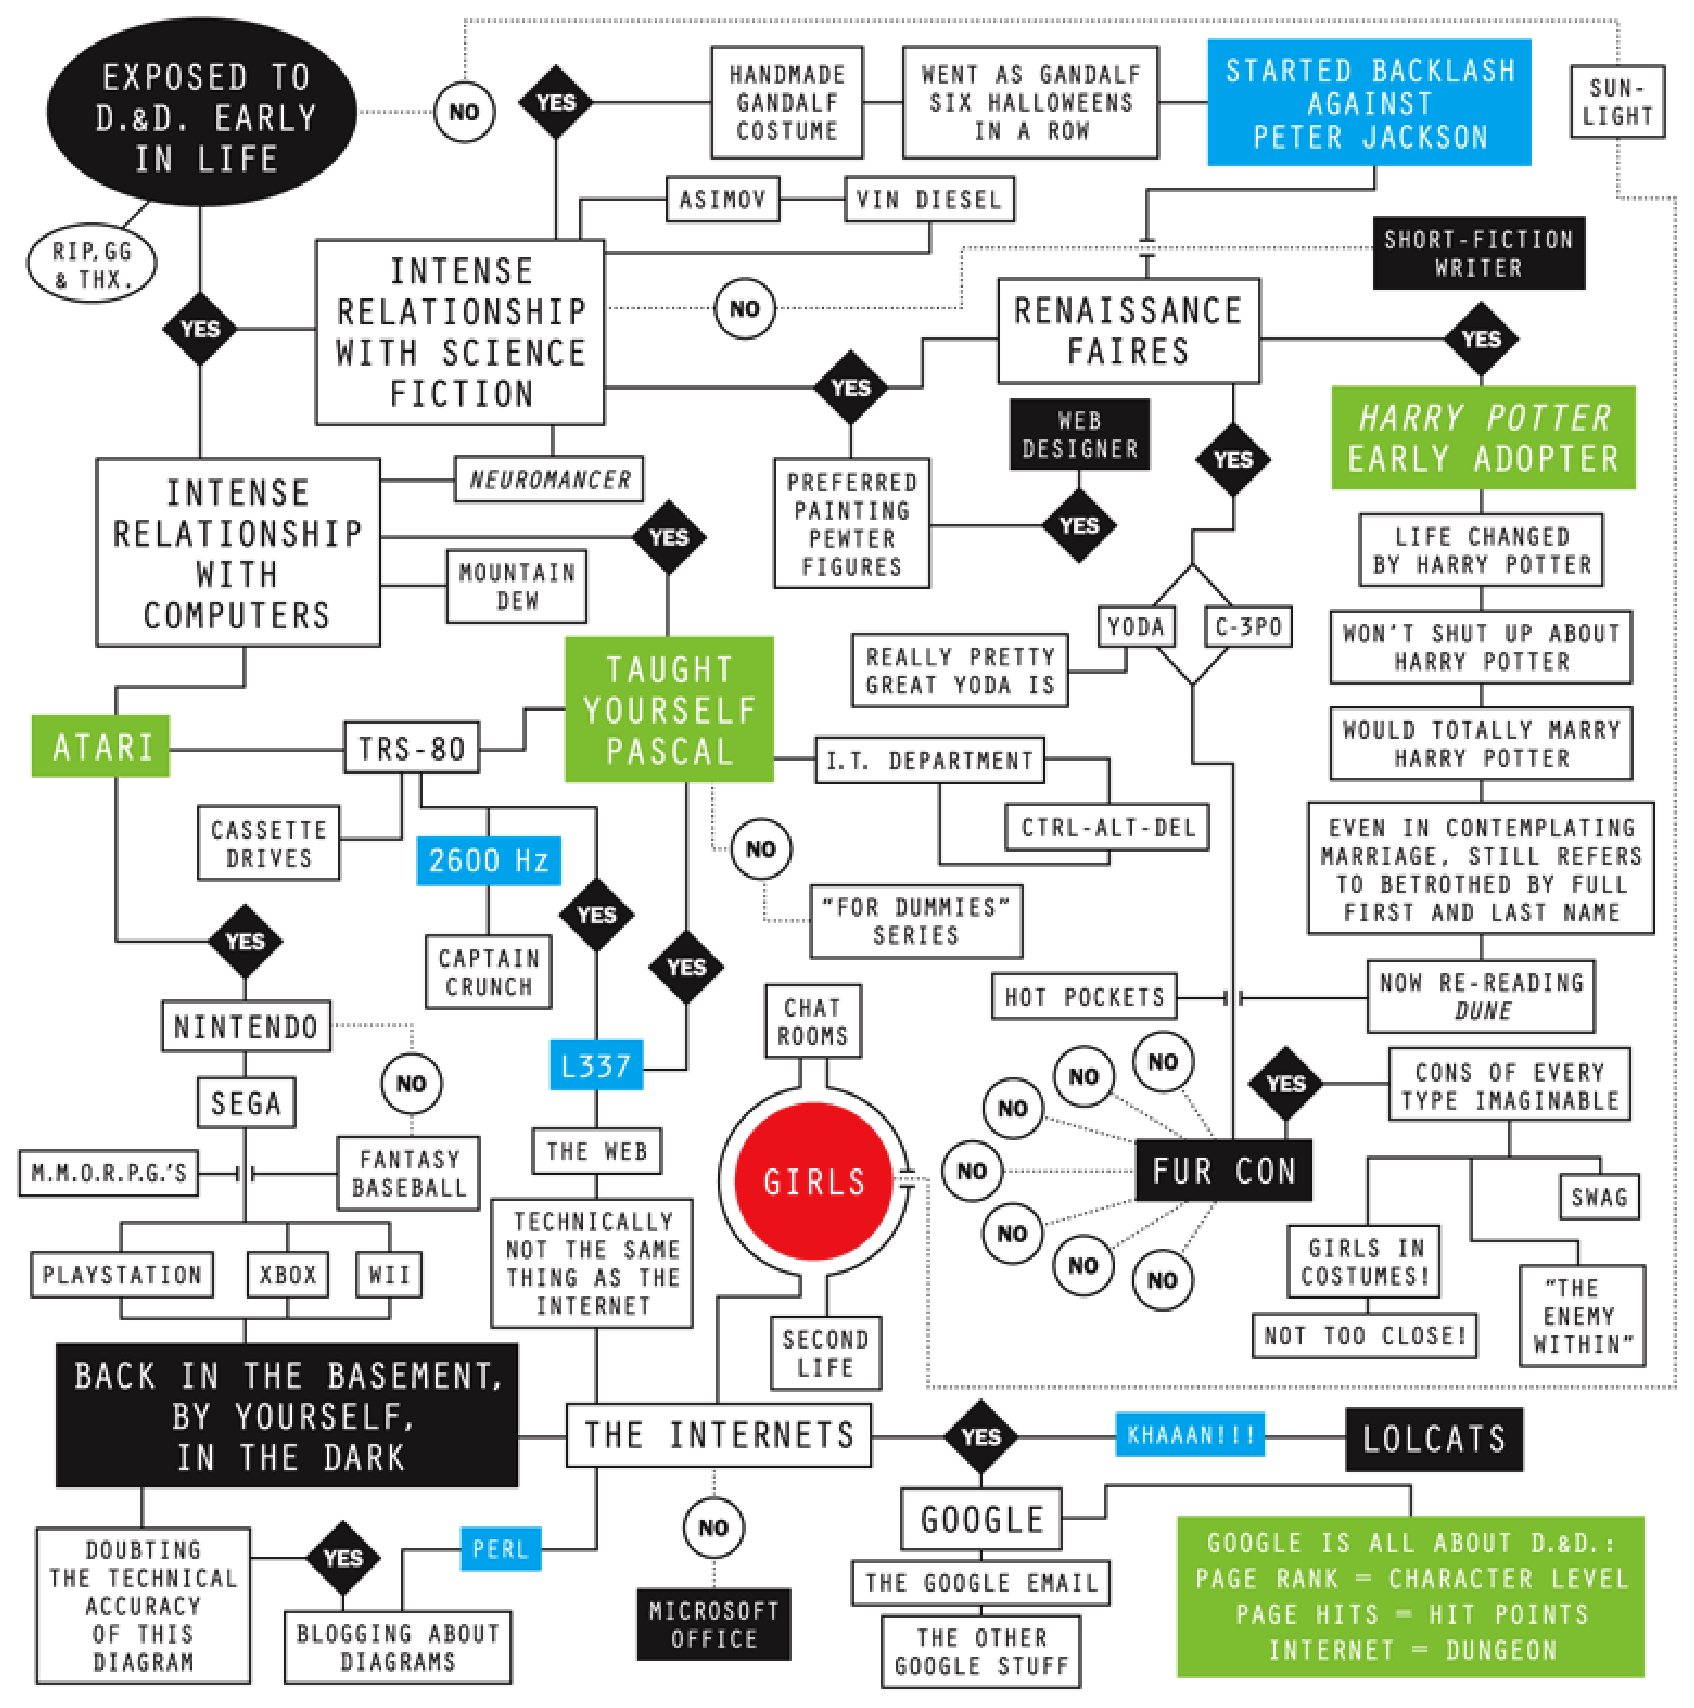
\includegraphics[width=0.7\textwidth]{\dir/figs/geek_flow_chart_nyt.eps}
%   \caption[first figure]{an example figure...}
%   \label{fig.example}
% \end{figure}

\section{The interaction between topology and branch lengths}
